\chapter{Extracción de normales a la superficie de una nube usando PCL}

\section{Introducción}
Se ha justificado en el capítulo anterior que será el algoritmo de extracción de vectores normales el que se llevará a hardware digital para ser optimizado. 

En este capítulo, se va a estudiar en profundidad dicho algoritmo exclusivamente en el ámbito de la librería PCL ya que ésta se sirve de librerías externas como son principalmente Eigen y boost. Este estudio es necesario para comprender cómo funciona el algoritmo y así poder realizar la optimización del hardware digital obtenido a partir de éste.

Por lo tanto, se explicará tanto en alto como en bajo nivel cómo PCL estima normales a la superficie de una nube de puntos de un modo semejante al que se ha utilizado para explicar fragmentos de código en capítulos anteriores.


\section{Técnica de estimación de vectores normales}

%http://mediatum.ub.tum.de/doc/800632/941254.pdf


Las normales a una superficie son de una de sus características geométricas más importantes no solamente en lo que concierne a la estimación de keypoints sino a otras áreas de computación gráfica como puede ser determinar las fuentes de luz adecuadas para generar sombras y brillos u otros efectos visuales semejantes. Por esta razón, la estimación de normales es una importante característica de la librería PCL.

Si se considera una superficie, normalmente es trivial estimar la dirección de la normal en un determinado punto como el vector perpendicular a la superficie en el mismo. Sin embargo, puesto que las nubes de puntos adquiridas por los sensores son un conjunto de puntos que representan una superficie, hay dos formas de proceder para estimar normales:

\begin{itemize}
\item[•]Reconstruir la superficie que representan los puntos utilizando técnicas de reconstrucción de superficies y entonces calcular los vectores a partir de la superficie reconstruida.
\item[•]Utilizar aproximaciones para estimar las normales directamente a partir de la nube de puntos.
\end{itemize}

Dada la complejidad que implica la primera opción, se va a proceder de ahora en adelante con la segunda, estimar vectores normales a partir de puntos que representan una superficie.

El problema de determinar un vector normal a una superficie en un punto de la misma se puede aproximar mediante una de las formas más simples y claras que se pueden plantear. Esto implica la estimación de la normal a un plano tangente a la superficie en el punto estudiado junto a $k$ puntos vecinos, siendo entonces $P^k$ el mencionado conjunto y un punto en particular $p_{i} \in P^{k}$ representado por sus coordenadas mediante $p_{i}=\left\lbrace p_{i_x},p_{i_y},p_{i_z} \right\rbrace$.

El plano utilizado para aproximar la normal en un punto de la nube es representado por un punto $x$ y un vector normal $\vec{n}$ de modo que la distancia de un punto $p_{i} \in P^{k}$ al plano queda definida como:

$$d_i=(p_{i}-x)\vec{n}$$

Además, $x$ se define como el centroide de $P^{k}$ de la siguiente manera:

$$x=\frac{1}{k}\sum_{i=1}^{k} p_i$$

Considerando lo anterior, se toman valores de $x$ y $\vec{n}$ de forma que, resolviendo un problema de mínimos cuadrados, $d_i$ sea cero para utilizar la mejor aproximación posible del plano tangente a la superficie de la nube en $p_i$.

Finalmente, la solución para $\vec{n}$ se da estudiando los autovectores y autovalores de la matriz de covarianzas $C \in R 3x3$ de $P^{k}$ calculada como:

$$C=\frac{1}{k}\sum_{i=1}^{k} (p_i-\bar{p})(p_i-\bar{p})^T,\;\;Cv_{j}=\lambda_ {j}v_{j},\;\;j \in \left\lbrace 0,1,2 \right\rbrace$$

$C$ es simétrica y semidefinida positiva con autovalores $\lambda_j \in R$ y autovectores $\vec{v_j}$.

Los autovectores son ortogonales entre sí y dan una aproximación de las principales componentes de $P^k$. No solo eso sino que si se cumple que:
 
 $$0\leq\lambda_1\leq\lambda_2\leq\lambda_3$$

entonces el autovector $v_0$, el cual se corresponde con el autovalor de menor valor $\lambda_0$, es una aproximación de $\vec{n}= \left\lbrace n_x,n_y,n_z\right\rbrace$, ventor normal a la superficie en el punto de la nube estudiado $p_i \in P^k$.


Debido a que no hay una forma estricta de calcular el signo del vector normal, su orientación es ambigua tras ser calculada con los procedimientos indicados anteriormente. Esto significa que las normales estimadas en la superficie de una nube de puntos no están consistentemente orientadas. Este efecto puede visualizarse en el ejemplo de la figura \ref{fig:normales_mal}.

La solución para este problema es trivial si se conoce la posición desde la cual se ha adquirido la nube, es decir, la posición del sensor. Para orientar todas las normales $\vec{n_i}$ hacia el punto de vista del sensor $v_p$ se debe cumplir:
$$\vec{n_i}(v_p-p_i)>0$$
Si se aplica esta corrección a la nube de la figura \ref{fig:normales_mal} se obtiene una orientación consistente de las normales tal y como se aprecia en la figura \ref{fig:normales_bien}.

\begin{figure}[!htb]
\minipage{0.48\textwidth}
  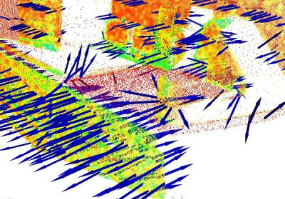
\includegraphics[width=\linewidth]{normales_mal}
  \caption{Vectores normales en una nube de puntos orientados de forma inconsistente.}\label{fig:normales_mal}
\endminipage\hfill
\minipage{0.48\textwidth}
  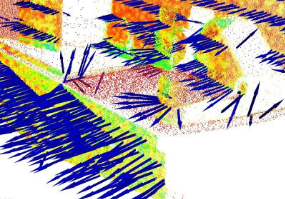
\includegraphics[width=\linewidth]{normales_bien}
  \caption{Vectores normales en una nube de puntos orientados de forma consistente.}\label{fig:normales_bien}
\endminipage\hfill
\end{figure}


\section{Estimación de normales a la superficie de una nube: alto nivel}
Conociendo el fundamento teórico relacionado con la estimación de normales a una superficie representada por un conjunto de puntos, se procede a continuación a explicar cómo PCL implementa este proceso.

Se retoma brevemente el código que permite calcular las normales en una nube de puntos:

\begin{lstlisting}[language=C++,breaklines]
  pcl::PointCloud<pcl::PointNormal>::Ptr cloud_normals (new 		pcl::PointCloud<pcl::PointNormal>);
  pcl::search::KdTree<pcl::PointXYZ>::Ptr tree_n(new pcl::search::KdTree<pcl::PointXYZ>());

  ne.setInputCloud(cloud_xyz);
  ne.setSearchMethod(tree_n);
  ne.setRadiusSearch(radius_search);
 
  std::cout << "Estimating normals in " << filename << " surface..." <<std::endl;

  begin = clock();
  ne.compute(*cloud_normals);
  end = clock();

  normal_estimation_time = double(end-begin)/CLOCKS_PER_SEC;
  std::cout << "Time needed for normal estimation (compute) in " << filename << ": " << normal_estimation_time << " seconds" << std::endl << std::endl;
\end{lstlisting}

Se recuerda que el método que lleva a cabo el algoritmo de estimación es $compute$ y cuyo contenido, explicado en alto nivel, es el que muestra el flujograma de la figura \ref{fig:compute_alto_nivel_diagram}.
Se ha tratado de resumir lo máximo posible la explicación de este algoritmo, obviando aspectos técnicos que no tienen cabida en este apartado y que se discutirán más adelante. 



\begin{figure}[!htb]
\centering
\minipage{0.6\textwidth}
  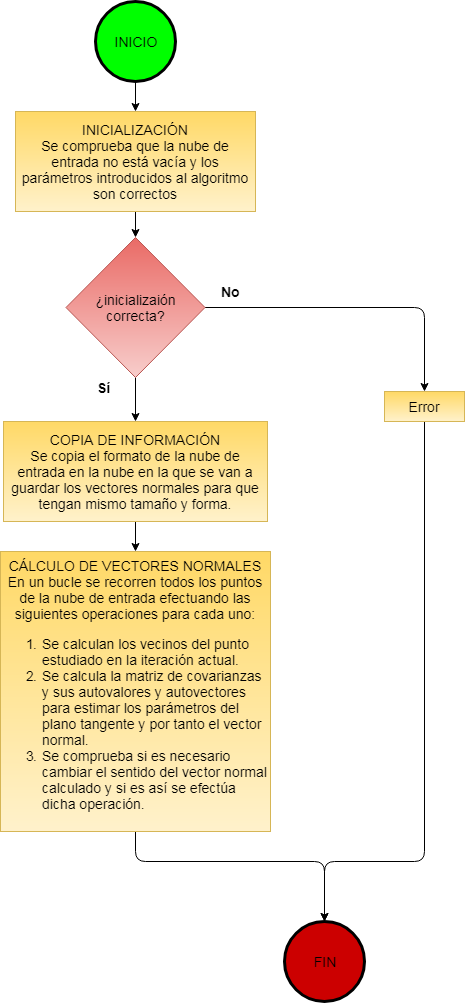
\includegraphics[width=\linewidth]{compute_alto_nivel_diagram}
  \caption{Proceso simplificado de estimación de normales en una nube de puntos.}\label{fig:compute_alto_nivel_diagram}
\endminipage\hfill

\end{figure}

\section{Estimación de normales a la superficie de una nube: bajo nivel}


\section{Conclusiones}
...

En el siguiente capítulo, se mostrarán las modificaciones pertinentes al algoritmo de estimación de normales para que sea sintetizable en hardware y se explicará el proceso de optimización llevado a cabo.
